\documentclass[ngerman]{scrartcl} 

\KOMAoptions{fontsize=12pt, paper=a4}
\KOMAoptions{DIV=11}
\usepackage[utf8]{inputenc}		% Direkte Eingabe von ä usw
\usepackage[T1]{fontenc}               	% Font Kodierung für die Ausgabe
\usepackage{babel}			% Verschiedenste sprach-spezifische Extras
\usepackage[autostyle=true]{csquotes}	% Intelligente Anführungszeichen
\usepackage{amsmath}		% Mathematischer Formelsatz mit zusätzlichen mathematischen Schriften und Symbolen
\usepackage{amssymb}		% Mathematischer Formelsatz mit zusätzlichen mathematischen Schriften und Symbolen
\usepackage{physics}			% Differentialgleichungen
\usepackage{listings}			% Zum Einbinden von Programmcode verwenden wir das listings-Paket
\usepackage[dvipsnames]{xcolor}	% um Elemente von Befehlen farblich zu unterstützen
\usepackage[varg]{txfonts}             	 % Schönere Schriftart
\usepackage{graphicx}		% Paket um externe Graphiken einzufügen
\RequirePackage[backend=biber, style=numeric]{biblatex} % Literaturverzeichnis
\usepackage{hyperref} 		% um klickbare Elemente in Ihrem PDF-Ausgabedokument zu erzeugen
\RequirePackage[all]{hypcap} 		% ergänzend zu hyperref
\usepackage{siunitx}			% Intelligentes Setzten von Zahlen und Einheiten
\usepackage{enumitem}		% Aufzählungsarten
\usepackage{fancyhdr}
\usepackage{float}			% Bild genau an der gewünschten Stelle [H] einfügen, 								% \begin{figure}[H]		\includegraphics[...]{{file name}}		\end{figure} 

\setlength\parindent{0pt} 		% Sets paragraph indentation to 0

\lstset{				% Deutsche Umlaute
	basicstyle=\ttfamily,    
	literate={~} {$\sim$}{1} 	% set tilde as a literal
	{ö}{{\"o}}1
	{ä}{{\"a}}1
	{ü}{{\"u}}1
	{ß}{{\ss}}1
	{Ö}{{\"O}}1
	{Ä}{{\"A}}1
	{Ü}{{\"U}}1
}
\lstset{
	numbers=left, 				% Line numbering
	numberstyle=\footnotesize, 			% Size of numbers
	basicstyle=\ttfamily\small, 			% Style and Size of Text
	backgroundcolor=\color{White}, 		% Background Color
	language=Python, 				% Language of Code
	commentstyle=\color{Maroon}, 			% Color and Style of Comments
	stringstyle=\color{OliveGreen}, 			% Color of Strings
	showstringspaces=false,
	morekeywords={import,from,class,def,for,while,if,is,in,elif,else,not,and,or,print,break,continue,return,True,False,None,access,as,del,except,exec,finally,global,import,lambda,pass,print,raise,try,assert}, 												% Definition of new keywords that will be highlighted
	keywordstyle=\color{RoyalBlue}			% Color and Style of Keywords
}


\pagestyle{fancy}
\fancyhf{}
\rhead{Ben Karcher, Annika Hoverath}
\lhead{Computerphysik - Abgabe 3}
\rfoot{Seite \thepage}


\begin{document}


\thispagestyle{fancy}

\section{H.7: Eigenwerte linearer Differentialoperatoren}
	Zunächst betrachten wir das folgende Randproblem:
	\begin{align*}
		u''(x) + g(x) u(x) &= 0\\
		u(t_0) &= u_0\\
		u(t_1) &= u_1
	\end{align*}
	Wenn wir nun die obige Gleichung mit Hilfe des linearen Differentialoperators $Du=u''+gu$ ausdrücken, lässt dich die DGL schreiben als: $Du=0$ (+ Randbedingungen) \\
	Vor allem suchen wir Pare aus Eigenwerten $\lambda$ und Eigenfunktionen $u_\lambda$, die die folgende Gleichung erfüllen:
	\begin{align}
		Du_\lambda=\lambda u_\lambda
	\end{align}
\subsection{Bedeutung der Eigenfunktion zu dem Operator D}
	In der ersten Teilaufgabe betrachten wir Eigenfunktionen des homogenen Systems mit homogenen Randbedingungen. 
	Diese sind von besonderer Bedeutung in der Lösung eines inhomogenen Systems mit Randbedingungen:
	\begin{align}
		D u(x) &= \lambda u(x) + f(x)\\
		u (t_0) &= a \nonumber\\
		u(t_1) &= b
	\end{align}
	Sei $u_{inhom}$ eine Lösung des inhomogenen Systems und $u_{hom}$ eine Lösung des homogenen Systems.
	Dann kann aus $u_{inhom}$ mit Linearkombinationen von $u_{hom}$ ein Lösungsschar konstruiert werden.
	\begin{align*}
		u &:=u_{inhom}+\alpha u_{hom}\\
		Du &= Du_{inhom}+\alpha Du_{hom}\\
		&= \lambda u_{inhom} + f+\alpha \lambda u_{hom}\\
		&= \lambda u + f\\
		u(t_0)&=u_{inhom}(t_0)+\alpha u_{hom}(t_0)=u_0\\
		u(t_1)&=u_{inhom}(t_1)+\alpha u_{hom}(t_1)=u_1
	\end{align*}
	$u$ ist also eine neue Lösung des inhomogenen Eigenwertproblems mit Randbedingungen.
\subsection{Spektrum von D}
	Nun bestimmen wir numerisch die 10 betragsmäßig kleinsten Werte im Spektrum von D für den Fall:
	\begin{align}
		g(x)&=0\\
		t_0=0 \quad&\&\quad u_0=0\nonumber\\
		t_1=60 \quad&\&\quad u_1=0\nonumber
	\end{align}
	Dies machen wir mit dem Numerov-Verfahren; eine Methode mit der man numerisch gewöhnliche Differentialgleichungen der Form $u''(x)=-g(x)u(x)+s(x)$ lösen kann.
	Die analytischen Lösungen können folgendermaßen bestimmt werden:
	\begin{align*}
		D u(x) - \lambda u(x) = 0 \Leftrightarrow u''(x) - \lambda u(x) = 0 \Leftrightarrow u''(x) = \lambda u(x)
	\end{align*}
	Wir behandeln also das folgende Gleichungssystem
	\begin{align}
		u''(x) &= \lambda u(x)\\
		u(0) &= 0\nonumber\\
		u(60) &= 0\nonumber
	\end{align}
	Dieses Gleichungssystem ist ein reguläres Sturm-Liouville-Problem. Dabei gibt es drei Fälle, die wir nun im Folgenden betrachten werden.
	\begin{itemize}
		\item $\lambda > 0$\\
			Wir wählen den Ansatz: $u(x) = e^{\alpha x}$. Setzen wir dies nun in Gleichung (5) ein, erhalten wir: 
			\begin{align*}
				u''(x) = \alpha^2 u(x) \Leftrightarrow \alpha^2 = \lambda \rightarrow \alpha = \pm \sqrt{\lambda}
			\end{align*}
			Damit haben wir die allgemeine Lösung gefunden: 
			\begin{align}
				u(x) = c_1 \cdot e^{\sqrt{\lambda} x} + c_2 \cdot e^{-\sqrt{\lambda} x}
			\end{align}
			Setzen wir nun die Randbedingungen ein, so erhalten wir: 
			\begin{align*}
				u(0) = c_1 + c_2 \overset{!}{=} 0 \rightarrow c_2 = - c_1\\
				u(60) = c_1 \cdot sinh(60 \sqrt{\lambda}) \overset{!}{=} 0
			\end{align*}
			Kein $\lambda$ kann diese Bedingung erfüllen. Somit sind alle $\lambda > 0$ keine Eigenwerte. 
		\item $\lambda = 0$\\
			In diesem Fall führt die Gleichung (5) zu der Form:
			\begin{align*}
				u''(x) = 0
			\end{align*}
				Somit ergibt sich $u(x)$ zu: $u(x) = c_1 x +c_2$. Nun folgen die Randbedingungen: 
			\begin{align*}
				u(0) \overset{!}{=} 0 = c_2 &\rightarrow c_2 = 0\\
				u(60) \overset{!}{=} 0= 60 \cdot c_1 &\rightarrow c_1 = 0
			\end{align*}
			Dies entspräche der trivialen Lösung. Somit ist $\lambda = 0$ ebenfalls kein Eigenwert. \newline
			Zu guter Letzt betrachten wir den Fall
		\item $\lambda < 0$\\
			Dieser Fall $u(x) = e^{\alpha x}$ verläuft analog zum ersten Fall $\lambda > 0$ mit der Änderung von:
			\begin{align*}
				\lambda = - \alpha^2 \rightarrow \alpha = \pm i \sqrt{|\lambda|}
			\end{align*}
			Somit lautet die allgemeine Lösung:
			\begin{align*}
				u(x) = A \cdot cos\left(x\sqrt{|\lambda|}\right) + B \cdot sin\left(x\sqrt{|\lambda|} \right)
			\end{align*}
			Setzen wir nun die Randbedingungen ein, so erhalten wir: 
			\begin{align*}
				u(0) \overset{!}{=} 0 &= A  \rightarrow A = 0\\
				u(60) \overset{!}{=} 0 &= B \cdot sin(60 \sqrt{|\lambda|})
			\end{align*}
			Da $B \neq 0$ sein muss (sonst hätten wir wieder die triviale Lösung), ergeben sich die Eigenwerte $\lambda$: 
			\begin{align*}
				\lambda = -\left(\frac{m \pi}{60}\right)^2
			\end{align*} mit $m \in \mathbb{N}$
			Somit sind alle Eigenwerte der DGL mit homogenen Randbedingungen negativ.
	\end{itemize}
	Nun betrachten wir den Fall mit inhomogenen Randbedingungen:
	\begin{align}
		u''(x) &= \lambda u(x)\\
		u(0) &= 1\nonumber\\
		u(60) &= 0\nonumber
	\end{align}
	Da die Differentialgleichung von zweiter Ordnung ist, können wir mit Hilfe des Numerov-Verfahrens für einen Anfangswert und Steigung genau eine Lösung finden. Wir definieren $u_{\lambda,s}$ durch:
	\begin{align*}
		u_{\lambda,s}(60)&=0\\
		u_{\lambda,s}'(60)&=s
	\end{align*}
	Da $D$ linear ist, sind skalierte Lösungen immer noch Lösungen. Also gilt unter Skalierung der Anfangswerte: 
	\begin{align}
		\alpha u_{\lambda,s}=u_{\lambda,(\alpha s)}
	\end{align}
	Nun suchen wir eine Lösungen zu den inhomogenen Randbedingungen (7). Dazu führen wir folgende Rechnung durch:
	\begin{align*}
		\delta:&=u_{\lambda,1}(0)\\
		\Rightarrow \frac{1}{\delta}u_{\lambda,1}(0)&=1\\
		\overset{(8)}{\Rightarrow}u_{\lambda,1/\delta}(0)&=1
	\end{align*}
	Folglich ist $u_{\lambda,1/\delta}$ die eindeutige Funktion, die das inhomogene Randwertproblem löst.
	Der Faktor $\frac{1}{\delta}$ divergiert genau dann, wenn $\delta \rightarrow 0$ läuft.
	Dies passiert, wenn $u_{\lambda,1}(0)=0$ ist. Also wenn $u_{\lambda,1}$ das homogene Problem löst.
	Wir plotten die Amplitude von dieser Lösung gegen $\lambda$ und lassen aus der Divergenz die Lösungen darstellen.
	\begin{figure}[htbp]
		\centering
		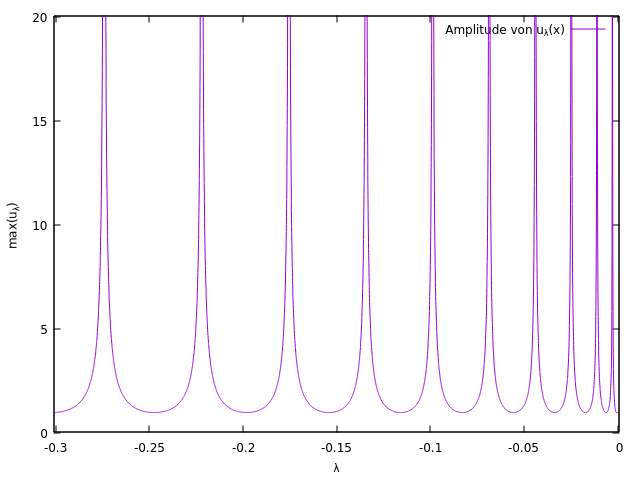
\includegraphics[width=0.8\textwidth]{code/amplitude_plot.png}
		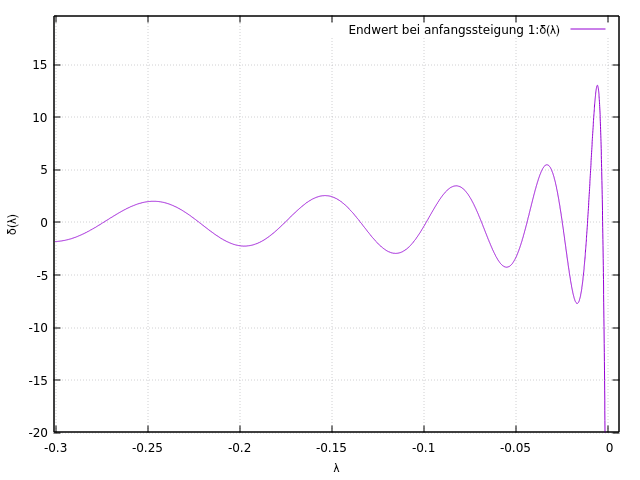
\includegraphics[width=0.8\textwidth]{code/endwert_plot.png}
		\caption[$f{ext}$]{
			Amplitude von $u_\lambda$ und $\delta(x)$ gegen $\lambda$.\\
			Wir sehen das $u_\lambda$ genau dann divergiert wenn $\delta(x)\rightarrow 0$
		}
		\label{fig:7}
	\end{figure}
	\newpage

\section{H.8: Kronig-Penney-Modell}
	In dieser Aufgabe betrachten wir die quantenmechanischen Zustände der Valenzelektronen eines kristallinen Festkörpers. Diese Elektronenzustände werden hier durch die Schrödingergleichung beschrieben:
	\begin{align}
		i\hbar \frac{\partial}{\partial t} \psi(t,x) = -\frac{\hbar^2}{2m_e} \Delta \psi(t,x) + V(x) \psi(t,x)
	\end{align}
	Dabei ist V(x) das Potential, welches durch die Ionen im Kristallgitter erzeugt wird. 
	Da sich die (stationären) Zustände mit der Zeit nicht verändern, sieht die Wellengleichung für ein Elektron im Kristall mit der Aufenthaltswahrscheinlichkeit ${|\Phi(x)|}^2$ nun folgendermaßen aus:
	\begin{align}
		\psi(t,x) = e^{-iEt/\hbar}\Phi(x)
	\end{align}
	Im Folgenden nehmen wir an, dass das Kristallgitter mit der Länge L ein endlicher Potentialtopf sei. Das periodische Potential im Eindimensionalen lautet:
	\begin{align}
		V_{per} = 60 (cos(\pi x))^{16}
	\end{align}
	Da wir nun annehmen, dass die Elektronen aus diesem unendlich hohen Potential durch die Wände bei $x = 0$ und $x = L$ nicht entkommen können, muss die Aufenthaltswahrscheinlichkeit an den Stellen $x = 0$ und $x = L$ null sein. Die Elektronen können ja nicht einfach aus dem Kristall tunneln (Annahme).
	Durch diese Randbedingungen ergibt sich das Potential zu:
	\begin{align}
		V(x)=\left\{\begin{array}{lll}
			\infty & x \leq 0\\
			V_{per}(x) & 0 < x < L\\
			\infty & x \leq L
		\end{array}\right. 
	\end{align}
\subsection{Energieeigenwerte}
	In dieser Teilaufgabe bestimmen wir nun mit Hilfe des Numerov-Verfahrens die Energieeigenwerte $\lambda$ für $L = 8$,
	wobei $0 \lesssim \lambda \lesssim max \{V_{per}(x)\}$ ist.
	Dazu bringen wir die homogene DGL in die folgende Form:
	\begin{align*}
		-\frac{1}{2}u''(x)+V(x)u(x)&=\lambda u(x)\\
		u''(x)&=-2(\lambda-V(x))\\
		u''(x)&=- g(x) u(x)+s(x)
	\end{align*}
	Mit $g(x):= 2(\lambda-V(x)),\quad s(x):=0$.\\
	Zusätzlich haben wir die Randbedingungen $u(0) = u(L) = 0$.
	Nach Gleichung (8) reicht es wieder für eine Anfangssteigung um die Differentialgleichung zu lösen.
	Wir definieren eine Funktion, die den Endwert einer Lösung mit Anfangssteigung 1 bestimmt:
	\begin{align}
		\delta(\lambda):= u_{\lambda,1}(60)
	\end{align}
	Diese wird im Programm "numerovError" benannt.
	Nullstellen von $\delta$ sind gerade die Eigenwerte zu dem homogenen Randwertproblem.\\
	Die so berechneten Eigenwerte könen benutzt werden um die Wellenfunktionen $\Phi_\lambda(x)$ zu besimmen.
	Datzu muss $u_\lambda(x)$ normiert werden aber da das problem homogen ist bleibt $\Phi_\lambda(x)$ eine Lösung.
	\begin{figure}[htbp]
		\centering
		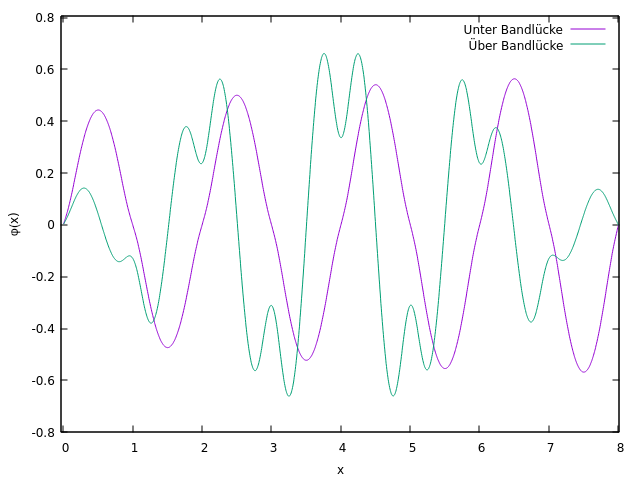
\includegraphics[width=0.8\textwidth]{code/wellen_plot.png}
		\caption[$f{ext}$]{
			Hier sehen wir zwei normierte Wellenfunktionen die die erste Bandlücke benachbarren.
			Beide sind Paritäts Eigenfunktionen um den punkt x=4; Eine mit positiver und eine mit negativer Parität.
		}
		\label{fig:8.1}
	\end{figure}
\subsection{Abhängigkeit der Bandstruktur von der Länge des Kristalls}
	Die Länge des Kristalls L ist im Vergleich zu einer realistischen Kristalllänge sehr viel kleiner.
	Deshalb überprüfen wir nun die Bandstruktur aus der vorherigen Aufgabe mit verschiedenen Längen L.
	Dabei setzen wir nun statt $L=8$ $L$ auf diverse Längen (siehe Plot).
	Damit wir die Abhängigkeit der Bandstruktur von der Kristalllänge L untersuchen können, bestimmen wir die Anzahl der Energiewerte und die Breite der Bandstruktur.\\
	Hierbei fällt uns auf, dass die Bandlücken sich nicht verschieben, aber die Anzahl an Eigenwerten zwischen jeder Lücke linear mit L wächst.
	In einem realen Kristall gibt es im Energiebereich der Bandlücke weitere lokale Zustände, die durch Verunreinigungen, Gitterfehler und Oberflächenfehler zustande kommen.
	Diesen Effekt lassen wir hier jedoch außen vor, da er für jedes Kristall individuell ist.
	Er ist abhängig von der Beschaffenheit des jeweiligen Kristalls. 
	\begin{figure}[htbp]
		\centering
		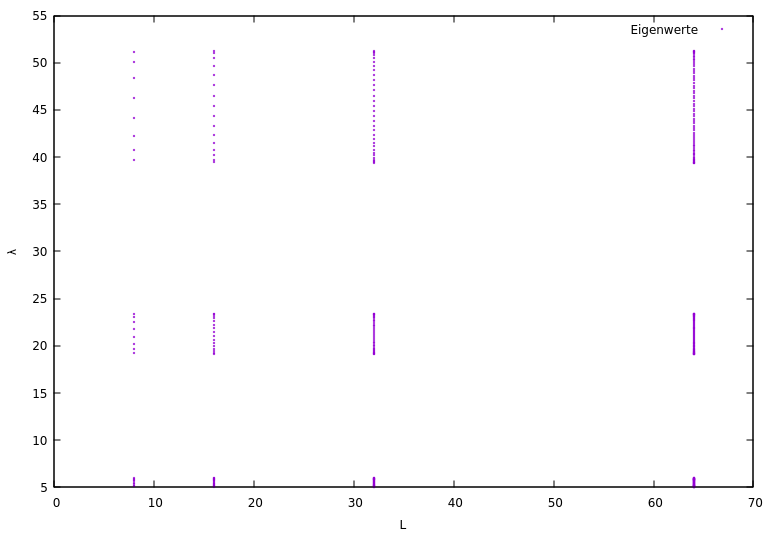
\includegraphics[width=0.8\textwidth]{code/L_plot.png}
		\caption[$f{ext}$]{
			Hier sind die Eigenwerte gegen L aufgetragen.
			Man sieht das die Bandlücken sich nicht verschieben aber die anzahl Eigenwerte linear wächst.
		}
		\label{fig:8.1}
	\end{figure}
\subsection{Kristall im äußere konstanten elektrischen Feld}
	Zu guter Letzt simulieren wir den Kristall in einem homogenen elektrischen Feld $- \epsilon$ mit dem Potential $V_e(x) = x \epsilon$.
	Die Funktion $g$ der Differentialgleichungen ändert sich zu: $g(x) = 2(\lambda - V(x) - V_e(x))$.
	Da wir geladene Teilchen in einem elektrischen Feld betrachten, werden die geladenen Teilchen im Kristallgitter aufgrund des äußeren Feldes verschoben.
	Durch das äußere elektrische Feld verschiebt sich die Aufenthaltswahrscheinlichkeit ${|\Psi(t,x)|}$ des Elektrons um den Atomkern.
	Dadurch entsteht im Inneren des Atoms eine makroskopisch inhomogene Ladungsverteilung.
	Dieses Phänomen nennt man "Verschiebungspolarisation".
	In dem Plot sieht man, dass die Eigenwerte durch das äußere Feld größer und zudem die Bandlücken kleiner werden.
	Die Bandlücken folgen den numerisch bestimmen Formeln:
	\begin{align*}
		\lambda_1&= 4.61\epsilon+12.64\pm(-5.38\epsilon+13.69)\\
		\lambda_2&= 4.65\epsilon+31.49\pm(-3.98\epsilon+16.85)
	\end{align*}
	\begin{figure}[htbp]
		\centering
		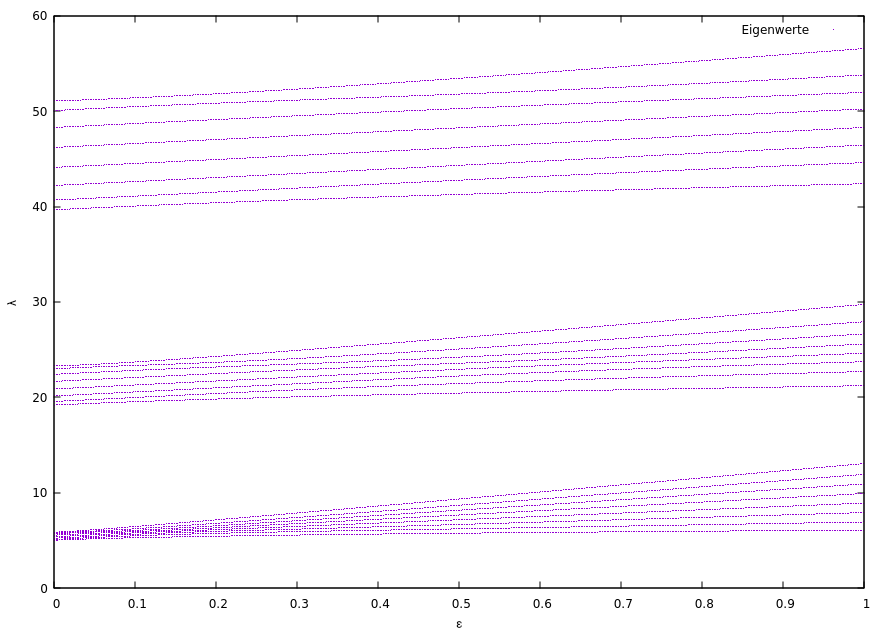
\includegraphics[width=0.95\textwidth]{code/epsilon_plot.png}
		\caption[$f{ext}$]{
			Hier sind die Eigenwerte gegen $\epsilon$ aufgetragen.
			Man sieht das die Bandlücken sich linear veschieben und verkleinern.
			}
		\label{fig:8.1}
	\end{figure}
\end{document}